\documentclass[uplatex, 12pt, a4paper, dvipdfmx]{jsarticle}
\title{}
\author{司馬博文 J4-190549\\hirofumi-shiba48@g.ecc.u-tokyo.ac.jp}
\date{\today}
\pagestyle{headings} \setcounter{secnumdepth}{4}
\usepackage{amsmath, amsfonts, amsthm, mathptmx, amssymb, ascmac, color, comment, graphicx}
\usepackage{tikz, tikz-cd}
\usepackage[top=15truemm,bottom=15truemm,left=10truemm,right=10truemm]{geometry}
\newtheorem{theorem}{定理} \newtheorem{definition}{定義} \newtheorem{proposition}{命題} \newtheorem{corollary}[proposition]{系} \newtheorem{lemma}[proposition]{補題}
\begin{document}
\maketitle

\begin{figure}[h] \caption{$v,V,V_a$間の関係を表すベクトル図} \label{fig2}
    \begin{center}
    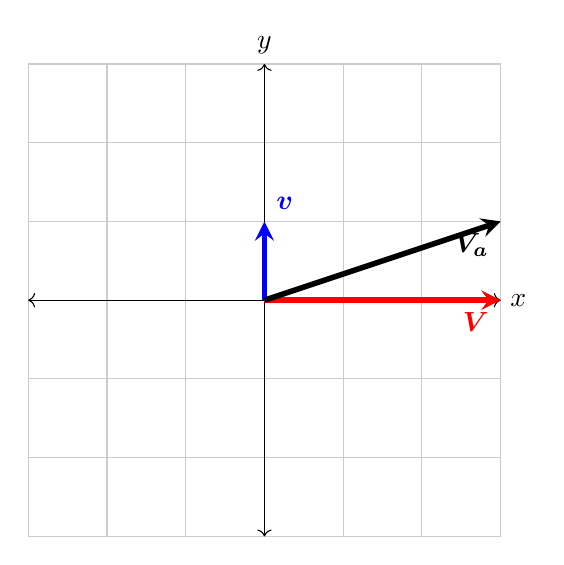
\begin{tikzpicture}
        \draw[thin,gray!40] (-3,-3) grid (3,3);
        \draw[<->] (-3,0)--(3,0) node[right]{$x$};
        \draw[<->] (0,-3)--(0,3) node[above]{$y$};
        \draw[line width=2pt,blue,-stealth](0,0)--(0,1) node[anchor=south west]{$\boldsymbol{v}$};
        \draw[line width=2pt,red,-stealth](0,0)--(3,0) node[anchor=north east]{$\boldsymbol{V}$};
        \draw[line width=2pt,black,-stealth](0,0)--(3,1) node[anchor=north east]{$\boldsymbol{V_a}$};
    \end{tikzpicture}
    \end{center}
    \end{figure}

    


\end{document}